\documentclass[12pt,oneside]{article}
\usepackage{makeidx,anysize,mflogo,xspace,float,epsfig,url}
\usepackage{amsmath,amsfonts,amssymb,a4wide} 
\usepackage[utf8]{inputenc}
%\usepackage[francais]{babel}
%\usepackage[french]{babel}
\urlstyle{sf}
%\usepackage{subcaption}
\usepackage{hyperref}
\usepackage{graphicx}
\usepackage{graphics}
\usepackage{float}
\usepackage{caption}
\usepackage{colordvi} %??
\usepackage{listings} 
\usepackage{subfigure}
\usepackage{subfloat}
\usepackage{xcolor}
\graphicspath{{./figures/}}
%\usepackage[labelsep=quad,indention=10pt]{subfig}
\definecolor{grey}{rgb}{0.95,0.95,0.95} % on définit la couleur grise
	% (c'est un gris très clair)
	\definecolor{red}{rgb}{1.0,0.0,0.0} 
	\definecolor{green}{rgb}{0.0,1.0,0.0}
	\definecolor{blue}{rgb}{0.0,0.0,1.0}
	\lstloadlanguages{bash,Java,C,C++,csh,make,sh}%%[Visual]Basic,xml}
	\lstset{frame=none,basicstyle=\footnotesize,breaklines,tabsize=2,captionpos=b,
		prebreak={\hbox{$\rightarrow$}},postbreak={\hbox{$\hookrightarrow$}},
		showstringspaces=false,backgroundcolor=\color{grey}\bfseries,
		keywordstyle=\color{blue},commentstyle=\color{green}\textit,
		stringstyle=\color{red}\ttfamily,abovecaptionskip=2pt,aboveskip=0pt,
		belowskip=0pt,belowcaptionskip=0pt,numbers=none,columns=fullflexible, backgroundcolor=\color{grey}}
%left,numberstyle=\footnotesize,
%		stepnumber=2,numbersep=1pt}

\begin{document}


\begin{center}
{\bf \Large Redpitaya: seventh example} \\ \ \\
G. Goavec-M\'erou, J.-M Friedt \\ \ \\ \today
\end{center}

This tutorial departs from the previous series in its aim of being portable to any
platform supported by the OscIMPDigital framework by not requiring dedicated hardware
peripheral to generate a data source but will rely on a pseudo-random generator to characterize
filter responses. By not requiring the ADC and DAC peripherals of the Redpitaya, this example
aims at demonstrating how assembling the blocks provided by this framework is portable
to various platforms including the ZC706 board or Altera-SoC based boards.

\begin{figure}[h!tb]
\begin{center}
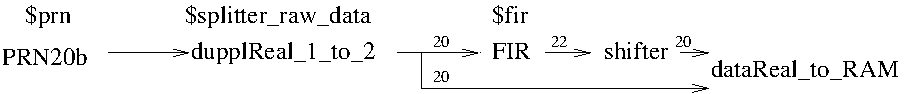
\includegraphics{schema}
\end{center}

\hspace*{-1.5cm}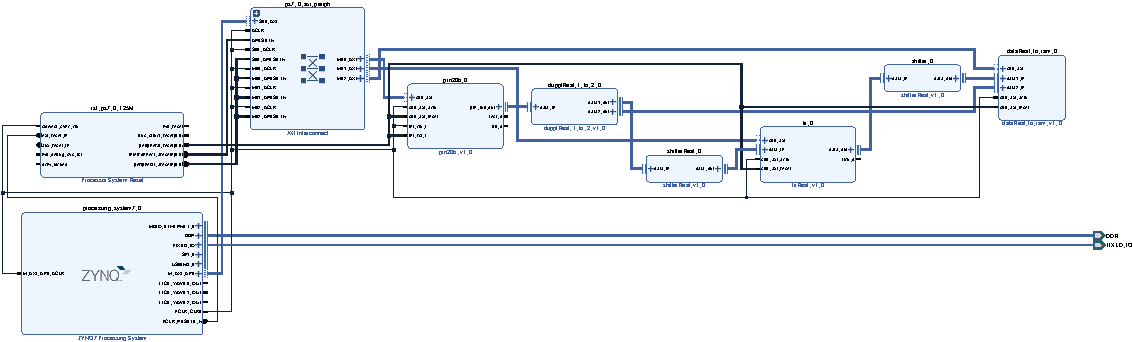
\includegraphics[width=1.2\linewidth]{design_1.pdf}
\caption{Schematic of the objective and final processing chain described in this document}
\label{fin}
\end{figure}

\section{PRN20 block}

Characterizing a filter response requires probing with a known source the device under test and
recording the response for each frequency. Assuming a linear, time invariant system, each
frequency can either be swept sequentially (frequency sweep network analyzer) or probed simultaneously
using a broadband noise generator and extracting each frequency contribution using a Fourier transform.
The latter approach is selected here, with the broadband noise generator being implemented as a
20-bit long linear feedback shift register (LFSR). With a repetition period of one million samples,
1~Msamples can be collected or a duration of 8~ms if clocking at a rate of 125~MHz. 

In the following example, the PRN output is fed to one channel of the Data to RAM block, and the
other channel goes through the filter with additional shifting to keep a controlled number of bits
before feeding the second channel of the Data to RAM block.

\section{PS: Linux kernel driver}

The same driver for communicating with the PL will be requested as
({\tt data\_to\_ram}), in addition to which we wish to communicate with
the FIR to configure taps. This time, the {\tt module\_generator} XML 
configuration file should look like

{\footnotesize
\begin{verbatim}
<?xml version="1.0" encoding="utf-8"?>
<drivers name="prn_fir" version="1.0">
  <driver name ="data_to_ram" >
    <board_driver name="data00" id="0" base_addr="0x43C20000" addr_size="0xffff" />
  </driver>
  <driver name ="fir" id="0" >
    <board_driver name="fir00"  id="0" base_addr="0x43C10000" addr_size="0xffff" />
  </driver>
</drivers>
\end{verbatim}
}

The name of the appropriate module has been found by looking for a directory
with the same name than the IP in the {\tt fpga\_driver} directory.

\begin{figure}[h!tb]
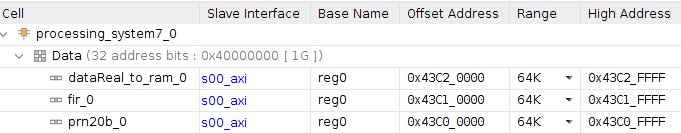
\includegraphics[width=\linewidth]{address}
\caption{Address range used by the IPs as defined by Vivado.}
\label{addr}
\end{figure}

In addition to displaying the graphical output of Vivado to find the address space used by
each block, we provide in {\tt design/addr.tcl} a Vivado TCL script for extracting such information
from the synthesized bitstream. Such a script is most useful when remotely working on a server
running Vivado without graphical display output. The output should look like

{\footnotesize
\begin{verbatim}
$ vivado -mode batch -source addr.tcl | grep -A1 \ SEG
NAME      string  false      SEG_dataReal_to_ram_0_reg0
OFFSET    string  false      0x43C20000
--
NAME      string  false      SEG_fir_0_reg0
OFFSET    string  false      0x43C10000
--
NAME      string  false      SEG_prn20b_0_reg0
OFFSET    string  false      0x43C00000
\end{verbatim}
}

\section{On the Redpitaya ...}

The userspace software is limited to configuring the FIR and collecting the raw data streamed
from the PRN generator as well as the filtered datastream.

\begin{lstlisting}[language=C]
#include <stdio.h>
#include <stdlib.h>
#include <stdint.h>
#include <fcntl.h>
#include <sys/types.h>
#include <sys/stat.h>
#include <unistd.h>
#include "fir_conf.h" // library for communicating with the FIR

int main()
{int k;
 char c[16384];
 int fi,fo;
 fi=open("/dev/data00",O_RDWR);
 fo=open("/tmp/data.bin",O_WRONLY|O_CREAT,S_IRWXU);
 fir_send_conf("/dev/fir00", "coefs.txt", 32);

 for (k=1;k<5;k++)
  {read(fi,c,16384);
   write(fo,c,16384);
  }
 close(fi);
 close(fo);
 return EXIT_SUCCESS;
}
\end{lstlisting}

The dataset is processed using the following GNU/Octave script

\begin{lstlisting}[language=C]
f=fopen('data15fois16.bin');d=fread(f,inf,'int32');x=d(1:2:end); 
z=zeros(1,length(x)); z(1:15)=1; 
u=(abs(fft(d(1:2:end)))); plot(u/max(u),'b'); hold on
u=(abs(fft(z-mean(z))));  plot(u/max(u),'r');
\end{lstlisting}

illustrating how the data are interleaved in the file ({\tt x=d(1:2:end);})
as well as the consistency of the filter shape with the expected transfer
function, here computed for the very simple rectangular window.

The results of the FIR filter implementation are illustrated in Figs. 
\ref{fir2} and \ref{fir1}). Fig. \ref{fir2} demonstrates the impact of the
FIR by displaying the power spectrum of the unfiltered data (blue, output
of the PRN generator) and filtered data (red) in the case of a simple
rectangular window filter. Fig. \ref{fir1} demonstrates the consistency
of the result with theory by overlaying the theoretical spectral response
of various rectangular window filters (red) with the experimental results
(blue).

\begin{figure}[h!tb]
\begin{center}
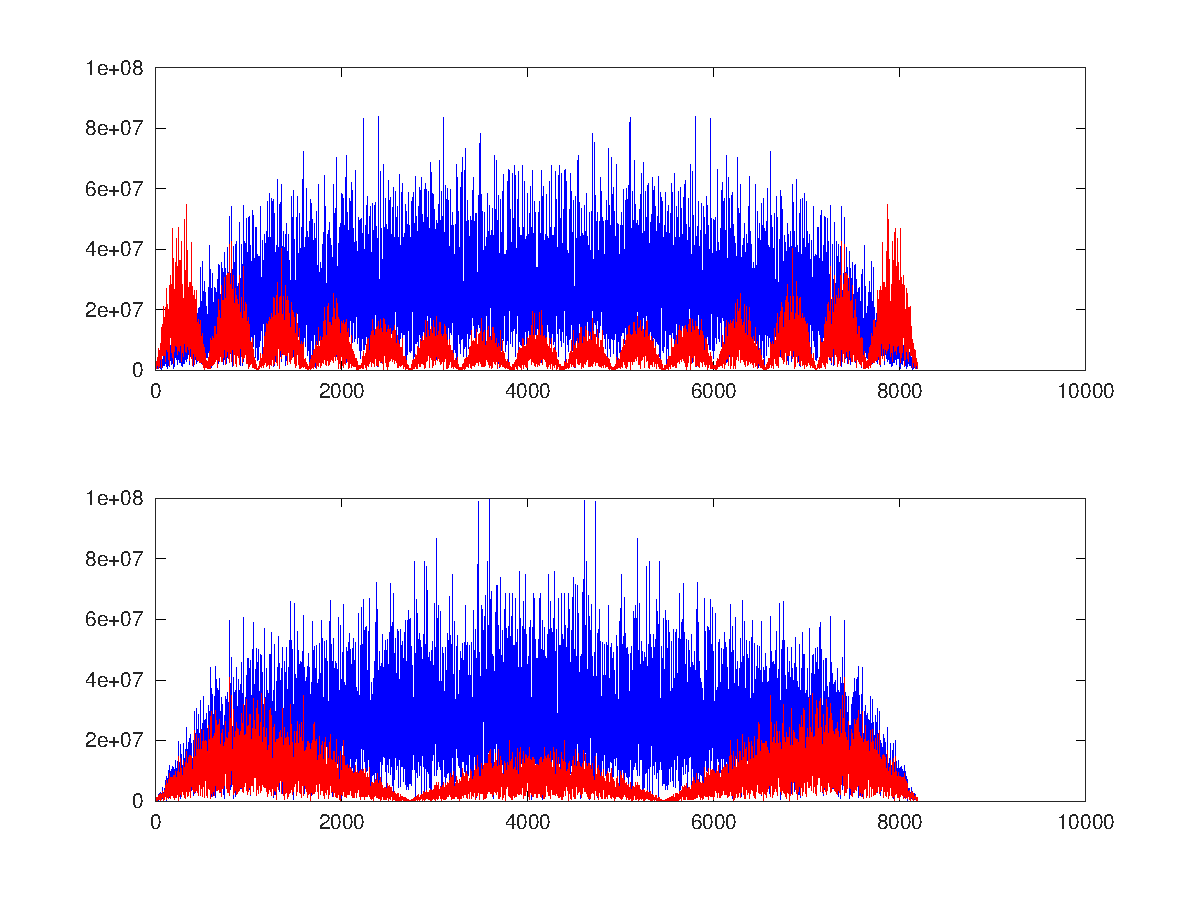
\includegraphics[width=.70\linewidth]{carac_fir2.pdf}
\end{center}
\caption{Comparison of the FIR input (pseudo random generator spectrum -- blue)
and the filtered output (red), here in the case of simple rectangular window 
filters.}
\label{fir2}
\end{figure}

\begin{figure}[h!tb]
\begin{center}
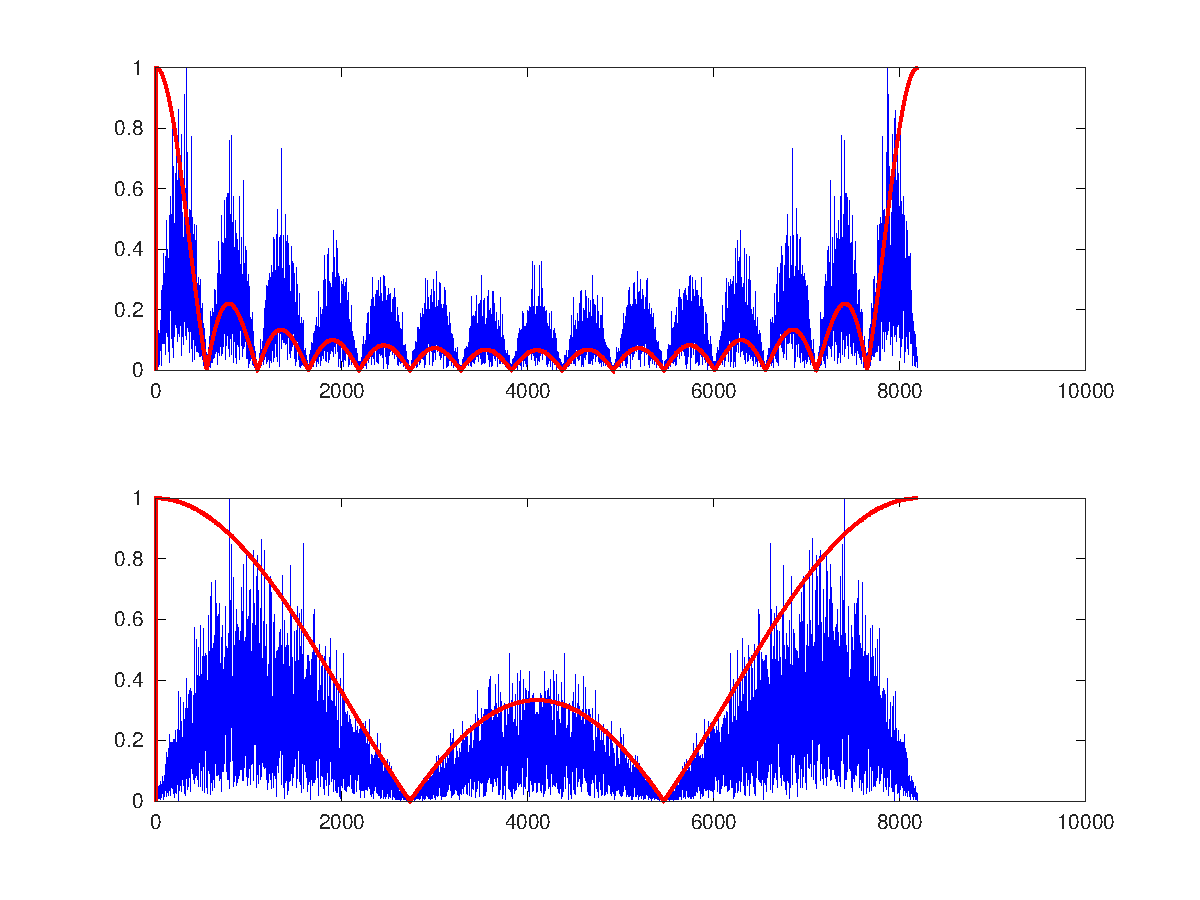
\includegraphics[width=.70\linewidth]{carac_fir1.pdf}
\end{center}
\caption{Comparison of the FIR filtered output (blue) and the expected filter
response (red), here in the case of simple rectangular window filters.}
\label{fir1}
\end{figure}
\end{document}
